% \documentclass[aspectratio=169]{beamer}
\documentclass[aspectratio=169, handout]{beamer}
 
\usepackage{algo}
\usepackage{sigmastyle}

\usepackage[backend=biber,style=authoryear,defernumbers=true]{biblatex}
\addbibresource{refs.bib}

\setbeamertemplate{blocks}[rounded]
\setbeamercovered{transparent}
\usecolortheme{orchid}
\usetheme{sigma}

\newcommand{\connected}{\texttt{Connected}}
\newcommand{\insertE}{\texttt{Insert}}
\newcommand{\removeE}{\texttt{Remove}}
\newcommand{\linkET}{\texttt{Link}}
\newcommand{\cutET}{\texttt{Cut}}
\newcommand{\findET}{\texttt{Find}}
\newcommand{\sizeET}{\texttt{Size}}
\newcommand{\TrueB}{\textsc{True}}
\newcommand{\FalseB}{\textsc{False}}
\renewcommand{\F}{\mathcal{F}}

\title{Dynamic Graph Connectivity}
\author{Ian Chen}
\date{}

\institute{University of Illinois Urbana-Champaign}

% --------------------------------------------------------------------

% Begin document
\begin{document}

\begin{frame}
    \titlepage
\end{frame}

\frame{\tableofcontents}

\section{Preliminaries}
\frame{\tableofcontents[currentsection]}

\begin{frame}{Problem Statement}
    \begin{itemize}
        \pause
        \item Queries:
              \begin{itemize}
                  \item $\connected(u, v)$, return whether there is a path between $u$ and $v$
                  \item $\connected(G)$, return whether $G$ is connected
              \end{itemize}
              \pause
        \item Updates:
              \begin{itemize}
                  \item $\insertE(u, v)$, add (undirected) edge $uv$ to the graph
                  \item $\removeE(u, v)$, remove edge $uv$ from the graph
              \end{itemize}
    \end{itemize}
\end{frame}

\begin{frame}{Example}
    \begin{enumerate}
        \item $\insertE(0, 1)$
              \pause
        \item $\insertE(2, 3)$
              \pause
        \item $\connected(0, 1) = \TrueB$
              \pause
        \item $\connected(0, 2) = \FalseB$
              \pause
        \item $\insertE(1, 2)$
              \pause
        \item $\connected(1, 3) = \TrueB$
              \pause
        \item $\removeE(2, 3)$
              \pause
        \item $\connected(2, 3) = \FalseB$
    \end{enumerate}
\end{frame}

\begin{frame}{Naive Methods}
    \begin{itemize}
        \item $O(1)$ update time, $O(m)$ query time?
              \pause
        \item $O(m)$ update time, $O(1)$ query time?
              \pause
        \item $O(\log^* m)$ insert time, $O(\log^* m)$ query time?
              \pause
              \only<4>{
                  \begin{itemize}
                      \item What about deletions?
                  \end{itemize}
              }
    \end{itemize}
\end{frame}

\begin{frame}{Bounds}
    \begin{itemize}
        \item $\max \set{t_{\text{update}}, t_{\text{query}}} = \Omega(\log n)$ \parencite{pǎtraşcu04-06}
              \pause
        \item $O(n^{1/2})$ update time, $O(1)$ queries \parencite{eppstein97-09}
              \pause
        \item Polylog update and query time \parencite{kapron13-01}
    \end{itemize}
\end{frame}


\section{Euler-Tour Trees}
\frame{\tableofcontents[currentsection]}

\begin{frame}{Spanning Trees and Forests}
    \begin{itemize}
        \item Represent each connected component with a \emph{spanning tree}
        \item A collection of spanning trees that contains every vertex is a \emph{spanning forest}
              \pause
        \item Answering queries is easy given a spanning forest supporting:
              \begin{itemize}
                  \item $\findET(u)$, find the root of the tree that $u$ is in
                  \item $\sizeET(u)$, number of nodes in the tree containing $u$
              \end{itemize}
              \pause
        \item $u, v$ connected iff $\findET(u) = \findET(v)$
        \item $G$ connected iff $\sizeET(v) = n$.
    \end{itemize}
\end{frame}

\begin{frame}{Linking and Cutting Trees}
    \begin{itemize}
        \item Change the spanning forest in a dynamic graph:
              \pause
        \item $\linkET(u, v)$, merge the trees $\findET(u)$ and $\findET(v)$
              \pause
        \item $\cutET(u, v)$, split the tree $\findET(u) = \findET(v)$ across $uv$
    \end{itemize}
\end{frame}

\begin{frame}{Euler Tours}
    \begin{itemize}
        \item An Euler-Tour is a closed walk that visits every edge exactly once.
              \pause
        \item An (undirected, connected) graph has an Euler-Tour if and only if every vertex has even degree
              \pause
        \item Trees never have Euler Tours (why?)
              \pause
        \item Doubling each edge, the tree has an Euler Tour
    \end{itemize}
\end{frame}

\begin{frame}[allowframebreaks]{Euler Tours on Trees}
    \begin{figure}
        
\includegraphics[height=0.65\textheight]{figs/s1.png}
        \caption{
            \textbf{Euler Tree on Trees:} (a) a spanning tree $T$ on $9$ nodes.
        }
    \end{figure}
    \begin{figure}
        
\includegraphics[height=0.65\textheight]{figs/s2.png}
        \caption{
            \textbf{Euler Tree on Trees:} (b) an Euler Tour on the tree $T$
        }
    \end{figure}
    \begin{figure}
        
\includegraphics[height=0.65\textheight]{figs/s3.png}
        \caption{
            \textbf{Euler Tree on Trees:} (c) Rotations of Euler Tour changes roots.
        }
    \end{figure}
    \begin{figure}
        
\includegraphics[height=0.65\textheight]{figs/s4.png}
        \caption{
            \textbf{Euler Tree on Trees:} (d) Subtrees are contiguous in Euler Tour.
        }
    \end{figure}
\end{frame}

\begin{frame}{Euler-Tour (ET) Trees}
    \begin{itemize}
        \item Represent the sequence as a self-balancing tree
              \pause
        \item $\findET(u)$
              \pause
              \begin{itemize}
                  \item $O(\log n)$ time; each node stores parent pointers
              \end{itemize}
        \item $\sizeET(u)$
              \pause
              \begin{itemize}
                  \item $O(\log n)$ time; each node stores size of its subtree
              \end{itemize}
        \item $\linkET(u, v)$
              \pause
              \begin{itemize}
                  \item $O(\log n)$ time; merge two trees and update sizes
              \end{itemize}
        \item $\cutET(u, v)$
              \pause
              \begin{itemize}
                  \item $O(\log n)$ time; remove edge from tree and update sizes
              \end{itemize}
    \end{itemize}
\end{frame}

\begin{frame}{Euler-Tour (ET) Trees}
    \begin{figure}
        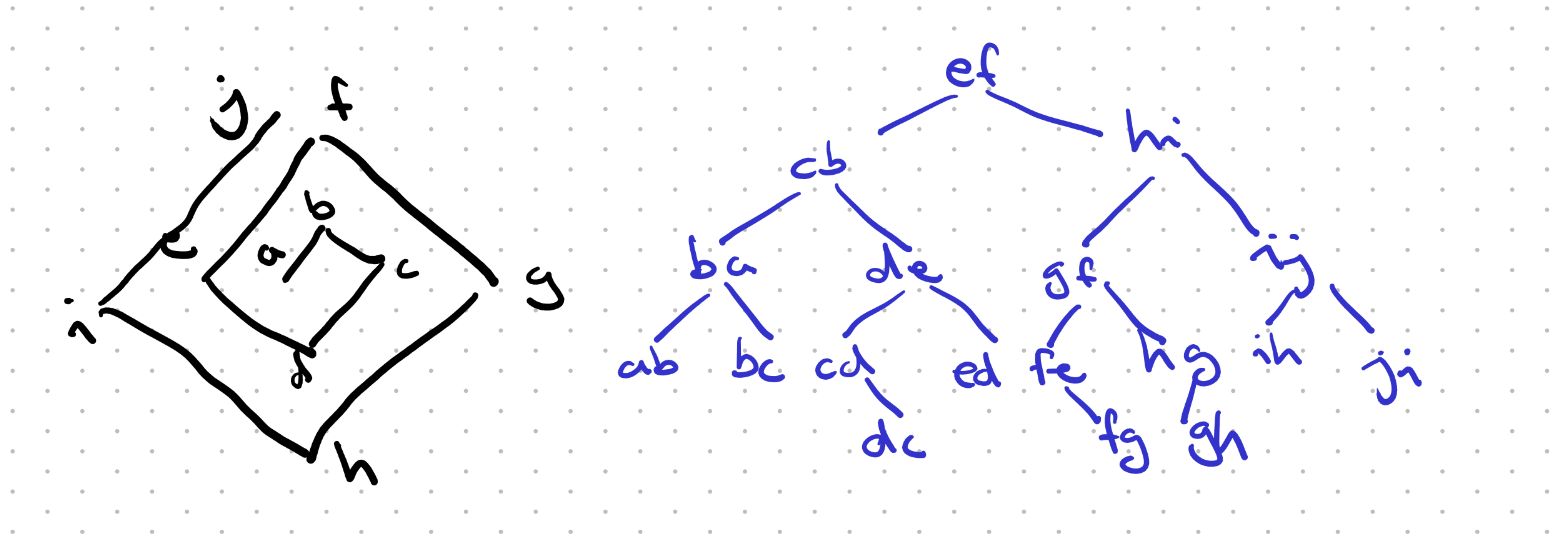
\includegraphics[height=0.45\textheight]{figs/s5.png}
        \caption{
            \textbf{ET Tree:} Left: a tree of depth $9$. Right: balanced tree representation of Euler Tour of depth $4$.
        }
    \end{figure}
\end{frame}

\begin{frame}{Inserting and Removing Edges}
    \begin{itemize}
        \item Upon $\insertE(u, v)$, use the $\linkET(u, v)$ operation
              \pause
        \item Upon $\removeE(u, v)$, use the $\cutET(u, v)$ operation to form $L$ and $R$ subtrees
              \pause
              \begin{itemize}
                  \item BUT, there may be another edge $u'v'$ connecting the $L$ and $R$
                        \pause
                  \item We must also call $\linkET(u', v')$
                        \pause
                  \item How do we check existence and find this connecting edge?
              \end{itemize}
    \end{itemize}
\end{frame}

\section{Dynamic Graph Connectivity}
\frame{\tableofcontents[currentsection]}

\begin{frame}{XOR Fingerprint}
    \begin{itemize}
        \item Let $\ell(v)$ label the vertices from $0, 1, \ldots, n-1$ with $\log_2(n)$ bits
              \pause
        \item Let $\ell(uv)$ (for $u < v$) be concatenation of label $[\ell(u), \ell(v)]$
              \pause
        \item Let $\F(v) = \bigoplus_{e \in N(v)} \ell(e)$ be the fingerprint of vertex $v$
              \pause
        \item For any $(S, \bar{S})$ cut of vertices:
              $$
                  \bigoplus_{v \in S} \F(v) = \bigoplus_{e \in E(S, \bar{S})} \ell(e)
              $$
              \pause
              \vspace{-\baselineskip}
        \item Computing $\bigoplus_{v \in S} \F(v)$ exactly the same as computing $\sizeET$
    \end{itemize}
\end{frame}

\begin{frame}{XOR Fingerprint (Continued)}
    \begin{itemize}
        \item If $E(L, R) = \emptyset$, then $\bigoplus_{v \in L} \F(v) = 0$
              \pause
        \item If $E(L, R) = \set{e}$, then $\bigoplus_{v \in L} \F(v) = \ell(e)$
              \pause
        \item How can we find an edge in $E(L, R)$ in general?
              \pause
              \only<4>{
        \item Find a \emph{subset} of $E$ with exactly one frontier edge
              }
    \end{itemize}
\end{frame}

\begin{frame}{Edgeset Sampling}
    \begin{itemize}
        \item Suppose $|E(L, R)| = \set{e_1, \ldots, e_k}$, with $2^i \le k < 2^{i+1}$
              \pause
        \item Let $E'$ be sampling edges iid with probability $2^{-i}$
              \pause
        \item $\Prob{|E'(L, R)| = 1} \ge 1/e^2 = \Theta(1)$
              \pause
              \only<4>{
                  \begin{align*}
                      \Prob{|E'(L, R)| = 1} & = k \Prob{e_1 \in E', e_2 \not \in E', \ldots, e_k \not \in E'}       \\
                                            & = (k) 2^{-i} (1 - 2^{-i})^k \ge (2^{i}) 2^{-i} (1 - 2^{-i})^{2^{i+1}} \\
                                            & = \left((1 - 2^{-i})^{2^{i}}\right)^2 \ge 1/e^2
                  \end{align*}
                  \vspace{-\baselineskip}
              }
              \pause
        \item Create $\log m$ independent sampling rates for each $i$
              \pause
        \item Create $O(\log n)$ independent copies to get high probability
    \end{itemize}
\end{frame}

\begin{frame}[allowframebreaks]{Kapron, King, Mountjoy Algorithm}
    \begin{figure}
        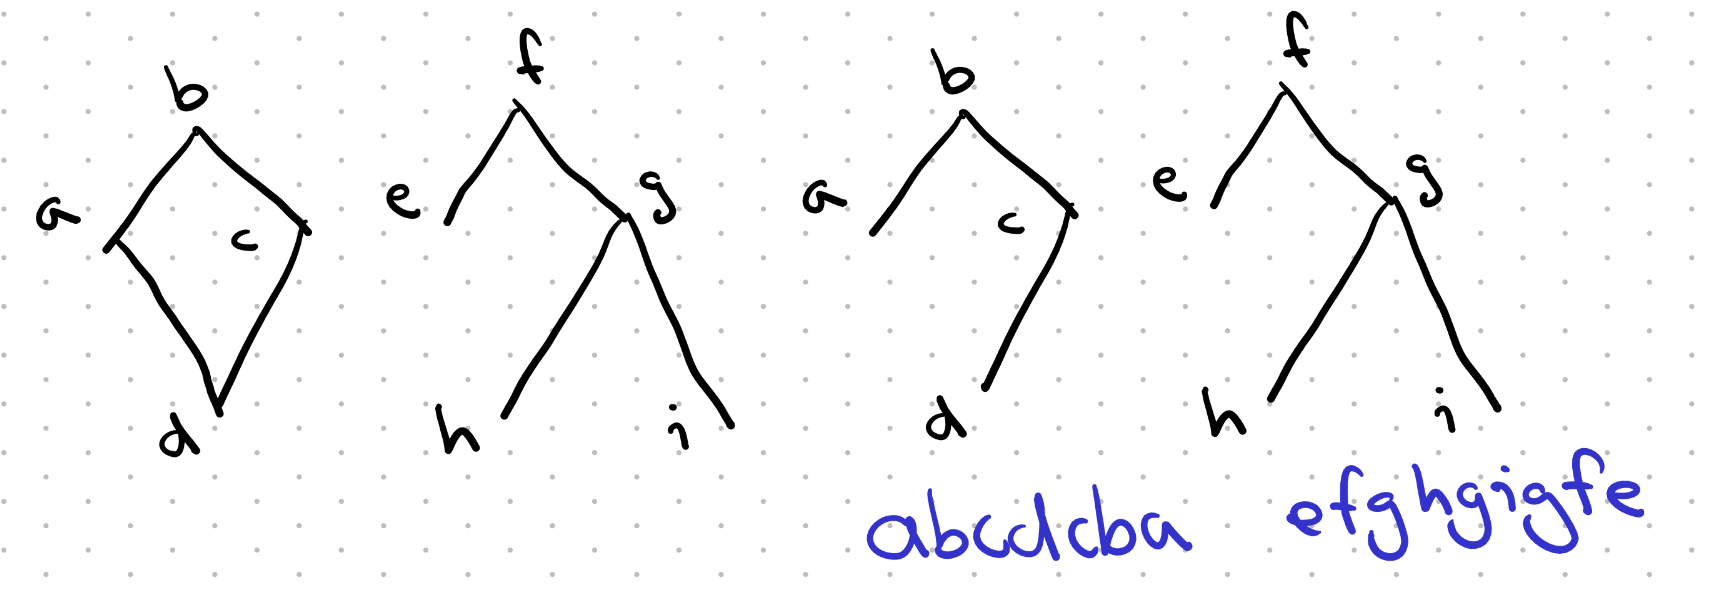
\includegraphics[width=\textwidth]{figs/s6.png}
        \caption{
            \textbf{KKM Algorithm:} (a) Left: graph $G$, Right: spanning forest $F$
        }
    \end{figure}
    \begin{figure}
        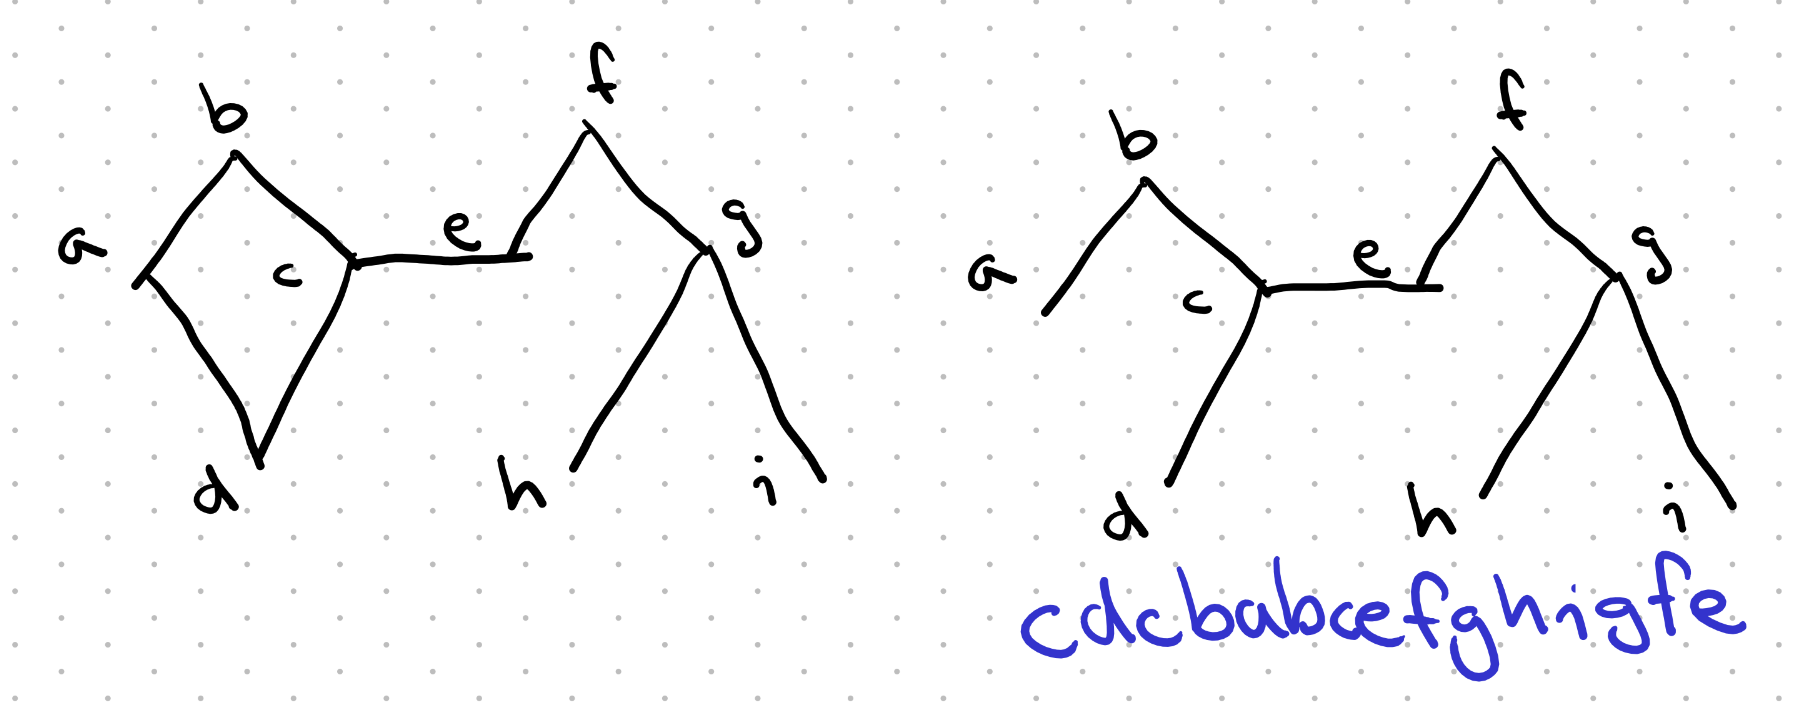
\includegraphics[width=\textwidth]{figs/s7.png}
        \caption{
            \textbf{KKM Algorithm:} (b) Insert edge $ce$ into $G$. $F$ becomes a single tree.
        }
    \end{figure}
    \begin{figure}
        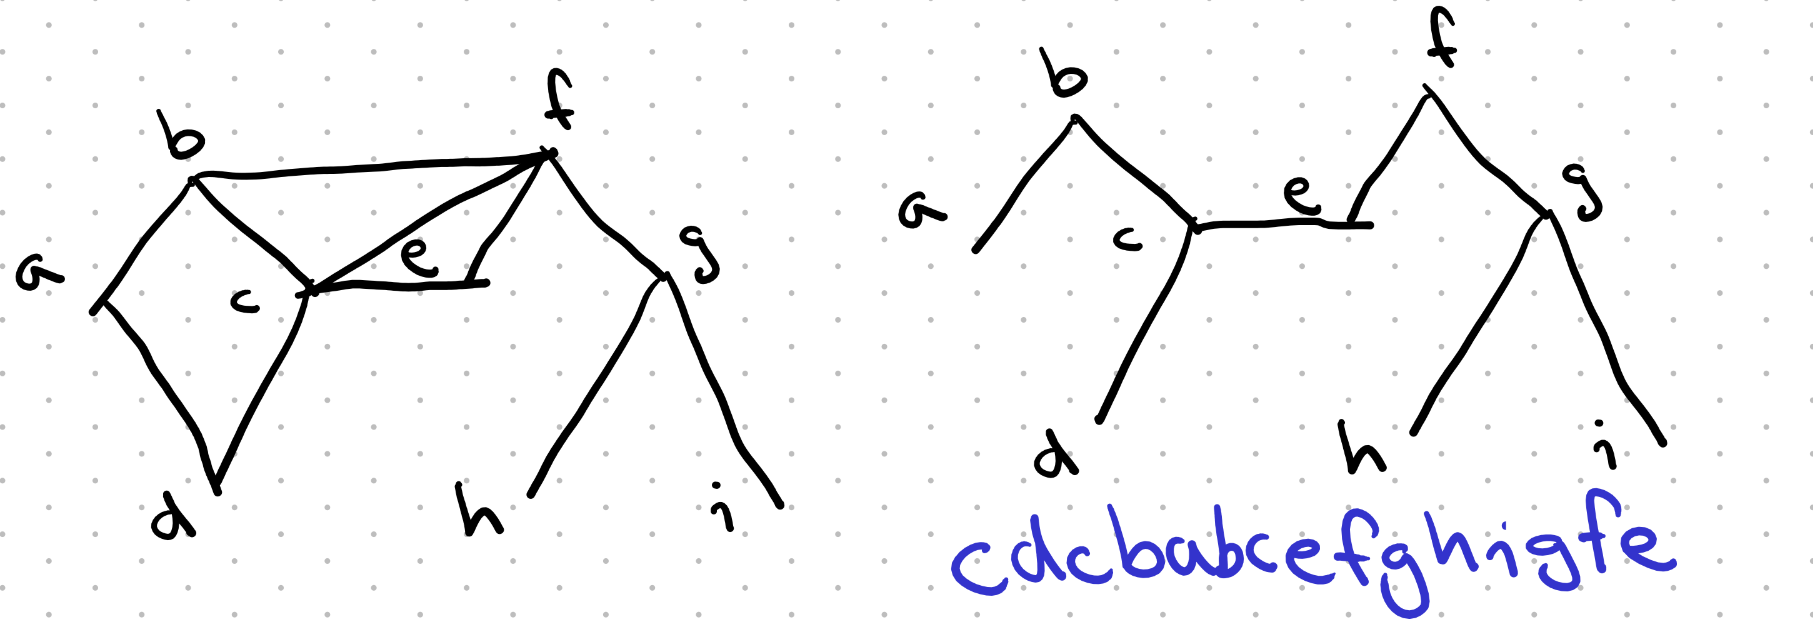
\includegraphics[width=\textwidth]{figs/s8.png}
        \caption{
            \textbf{KKM Algorithm:} (c) Insert edges $cf$ and $bf$. $F$ does not change.
        }
    \end{figure}
    \begin{figure}
        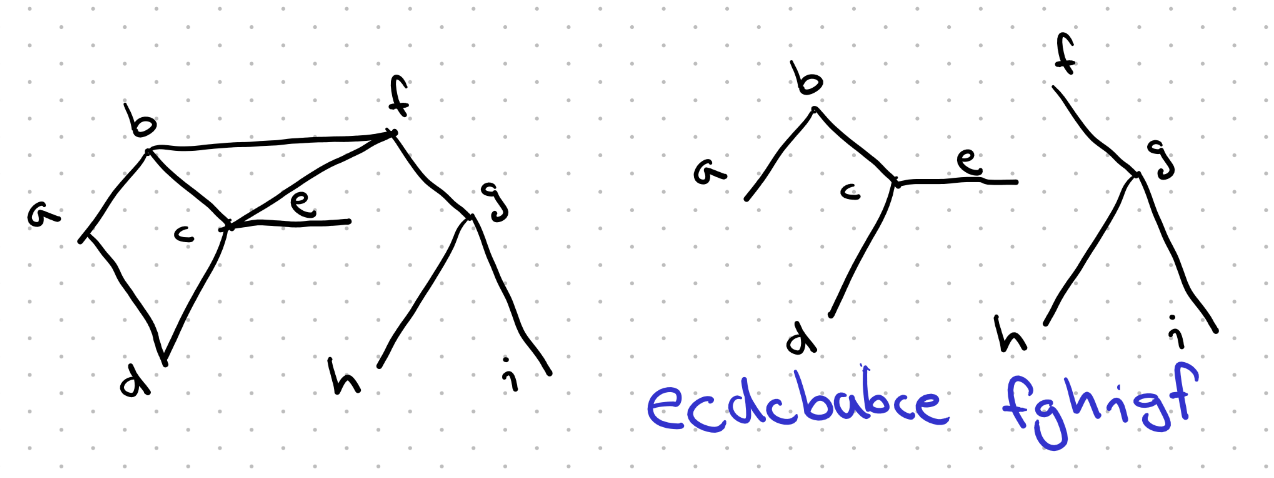
\includegraphics[width=\textwidth]{figs/s9.png}
        \caption{
            \textbf{KKM Algorithm:} (d) Remove edge $ef$. $F$ cut into $abcde$ and $fghi$.
        }
    \end{figure}
    \begin{figure}
        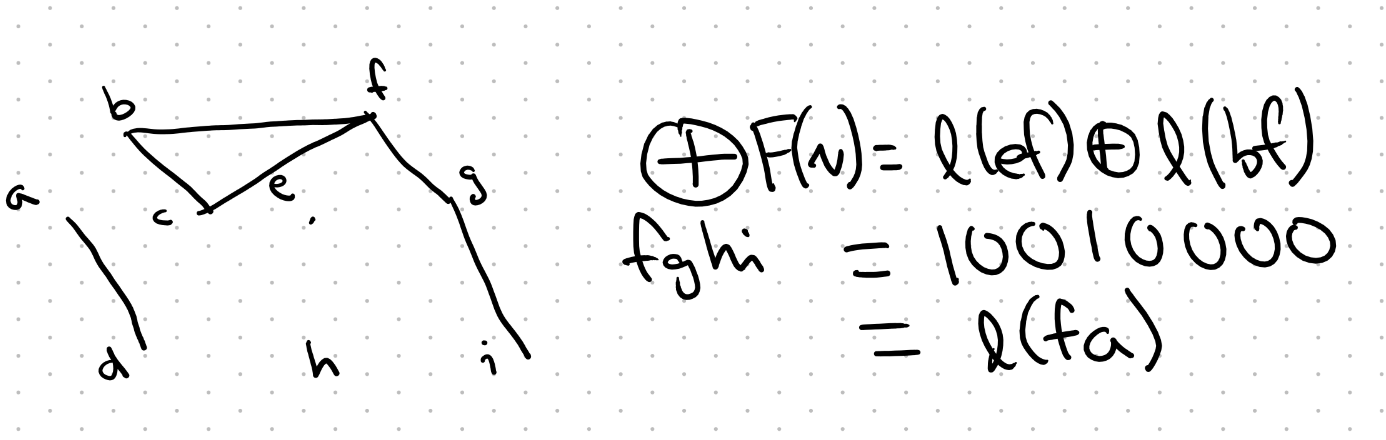
\includegraphics[width=\textwidth]{figs/s10.png}
        \caption{
            \textbf{KKM Algorithm:} (e) Fingerprints on subsampled edge set $E_1$.
            Fingerprint finds to find replacement edge $fa$ not in $E$, so \textsc{Fail}.
        }
    \end{figure}
    \begin{figure}
        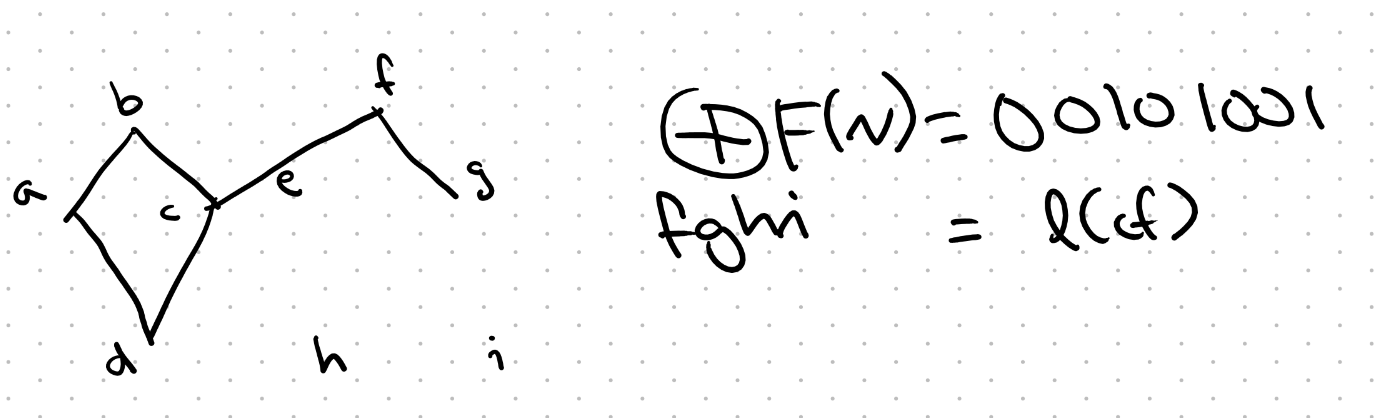
\includegraphics[width=\textwidth]{figs/s11.png}
        \caption{
            \textbf{KKM Algorithm:} (f) Fingerprints on subsampled edge set $E_2$.
            Fingerprint finds to find replacement edge $cf$ in $E$, so \textsc{Success}.
            Links forest back into one tree along $cf$.
        }
    \end{figure}
\end{frame}

\begin{frame}[allowframebreaks]{Bibliography}
    \nocite{pǎtraşcu04-06}
    \nocite{kapron13-01}
    \nocite{eppstein97-09}
    \printbibliography
\end{frame}

\end{document}
